\documentclass{article}
\usepackage[a4paper, tmargin=1in, bmargin=1in]{geometry}
\usepackage[utf8]{inputenc}
\usepackage{graphicx}
\usepackage[justification=centering]{caption}

% \usepackage{parskip}
\usepackage{pdflscape}
\usepackage{listings}
\usepackage{hyperref}
\usepackage{caption}
\usepackage{subcaption}
\usepackage{float}
\usepackage{enumerate}
\usepackage{amsmath}

\setlength{\parindent}{0pt}

\title{CS 754 : Advanced Image ProcessingAssignment 4}
\author{Meet Udeshi - 14D070007\\
  Arka Sadhu - 140070011\\
}
\date{\today}

\newcommand{\lone}[1]{
  ||#1||_{l_1}
}
\newcommand{\ltwo}[1]{
  ||#1||_{l_2}
}
\newcommand{\linf}[1]{
  ||#1||_{l_\infty}
}

\begin{document}
\maketitle
\section*{Q1}
\subsection*{A1.1 Derivatives for Calculation of Gradient Descent}
The given cost function is
\begin{equation}
  \label{eq:1}
  E(W,{h_i}) = \sum_{i=1}^N\sum_{j=1}^n(-y_{ji}log(Wh_i)_j + (Wh_i)_j) + \lambda\sum_{k=1}^K\sum_{j=1}^Nh_{kj}
\end{equation}

\begin{itemize}
\item Gradient of W:\\
  We note to get the gradient of a matrix, we need to differentiate with respect to every element of the matrix. The gradient matrix will simply be derivative to of the cost function with respect to the correspoding element of $W$.

  Let us consider the derivative with respect to the $a^{th}$ row and $b^{th}$ column denoted by $w_{ab}$.
  $$[\nabla W]_{ab} = \frac{dE}{dw_{ab}}$$
  $$\frac{dE}{dw_{ab}} = \frac{d}{dw_{ab}}(\sum_{i=1}^N\sum_{j=1}^n(-y_{ji}log(Wh_i)_j + (Wh_i)_j) + \lambda\sum_{k=1}^K\sum_{j=1}^Nh_{kj})$$
  We note that
  $$(Wh_i)_j = \sum_{l=1}^KW_{jl}h_{li}$$
  Clearly the last term of the cost function is not dependent on $W$ and hence goes to zero. For the first term we need to consider only the $a^{th}$ row
  $$\frac{dE}{dw_{ab}} = \frac{d}{dw_{ab}}(\sum_{i=1}^N(-y_{ai}log(Wh_i)_a + (Wh_i)_a)$$
  Consider the first term
  $$\frac{d}{dw_{ab}}\sum_{i=1}^N(-y_{ai}log(Wh_i)_a) = \sum_{i=1}^N \frac{d}{dw_{ab}}(-y_{ai}log(\sum_{l=1}^KW_{al}h_{li})) =
  \sum_{i=1}^N -\frac{y_{ai}}{(Wh_i)_a}(h_{bi})$$
  Now consider the second term
  $$\frac{d}{dw_{ab}}\sum_{i=1}^N(Wh_i)_a = \sum_{i=1}^N h_{bi}$$
  Therefore
  $$\frac{dE}{dw_{ab}} = \sum_{i=1}^N -\frac{y_{ai}}{(Wh_i)_a}(h_{bi}) + h_{bi} = \sum_{i=1}^N(1-\frac{y_{ai}}{(Wh_i)_a})h_{bi}$$
  We vectorize the equaiton for matlab as follows
  % $$ywh = Y./(WH)$$
  $$[\nabla W] = (1 -Y./WH)H^{'}$$

\item Gradient of H:\\
  We follow similar strategy to get the gradient of $H$. We differentiate the cost with respect to each of the elements of the matrix $H$. We denote the element at row $a$ and column $b$ by $h_{ab}$
  $$[\nabla H]_{ab} = \frac{dE}{dh_{ab}}$$
  $$\frac{dE}{dh_{ab}} = \frac{d}{dh_{ab}}(\sum_{i=1}^N\sum_{j=1}^n(-y_{ji}log(Wh_i)_j + (Wh_i)_j) + \lambda\sum_{k=1}^K\sum_{j=1}^Nh_{kj})$$
  We consider the three terms separately. For the first term we will need to consider only the $b^{th}$ column of H. 
  $$\frac{d}{dh_{ab}}\sum_{j=1}^n -y_{jb}log(\sum_{l=1}^KW_{jl}h_{lb}) = \sum_{j=1}^n-\frac{y_{jb}}{Wh_b}_jW_{ja}$$
  For second term also we consider only $b^{th}$ column
  $$\sum_{j=1}^n \frac{d}{dh_{ab}}\sum_{l=1}^KW_{jl}h_{lb} = \sum_{j=1}W_{ja}$$
  The third term will simply be $\lambda$
  Therefore
  $$\frac{dE}{dh_{ab}} = (\sum_{j=1}^n-\frac{y_{jb}}{Wh_b}_jW_{ja} + W_{ja}) + \lambda$$
  We vectorize the equation for matlab as follows
  $$[\nabla H] = W'*(1 - Y./WH) + lambda$$
  
  
\end{itemize}

\section*{Results}

\textbf{Parameters:}\\
\\
$ \lambda = 20 $\\
\\
Initial step size = 0.1\\
\\
Iterations = 200\\

\subsection*{Peak = 30}
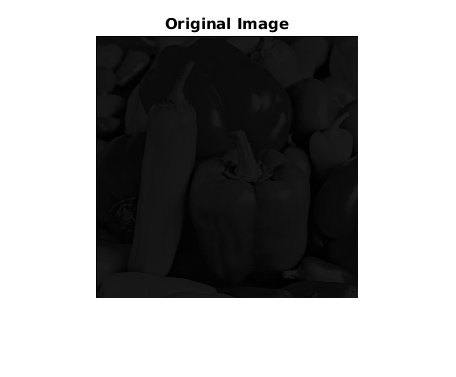
\includegraphics[scale=0.5]{images/peak30_orig}
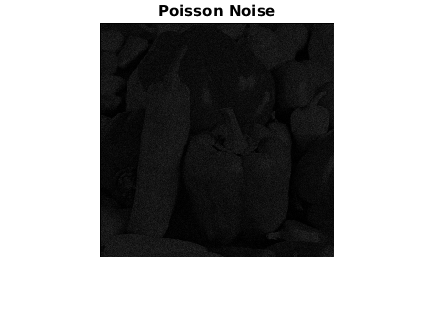
\includegraphics[scale=0.5]{images/peak30_noisy}
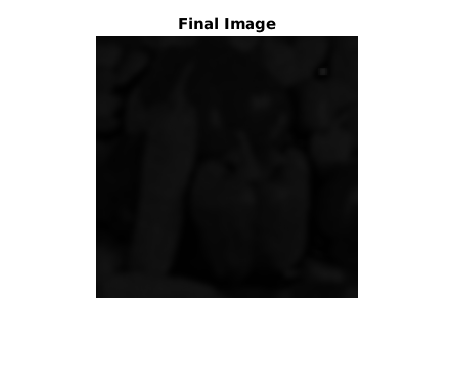
\includegraphics[scale=0.5]{images/peak30_denoised}
\\
PSNR\textsubscript{denoised} = 18.097 dB\\
\\
PSNR\textsubscript{noisy} = 13.920 dB

\subsection*{Peak = 60}
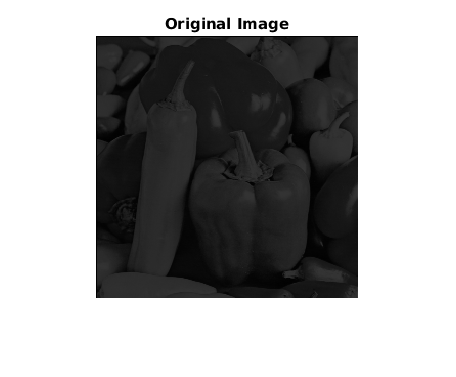
\includegraphics[scale=0.5]{images/peak60_orig}
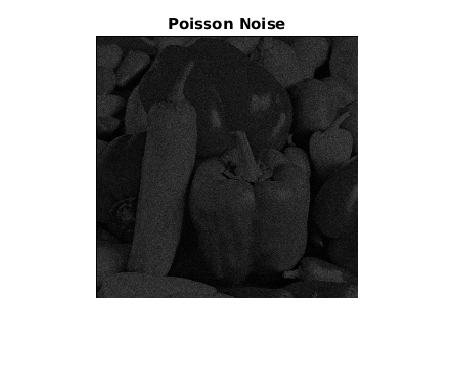
\includegraphics[scale=0.5]{images/peak60_noisy}
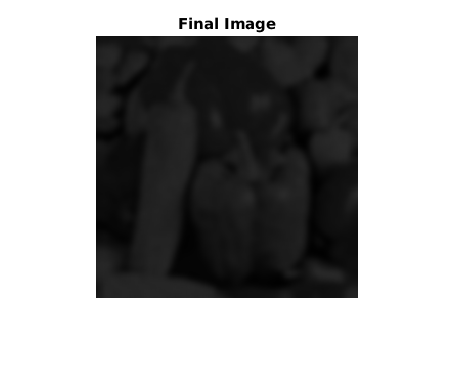
\includegraphics[scale=0.5]{images/peak60_denoised}
\\
PSNR\textsubscript{denoised} = 20.162 dB\\
\\
PSNR\textsubscript{noisy} = 16.825 dB

\subsection*{Peak = 100}
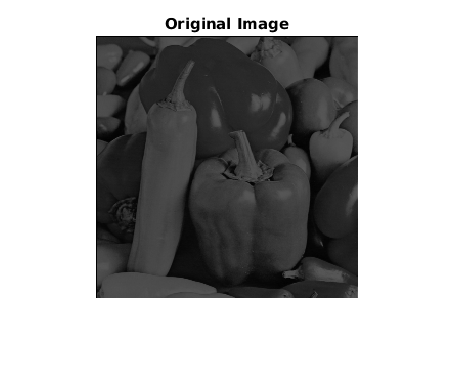
\includegraphics[scale=0.5]{images/peak100_orig}
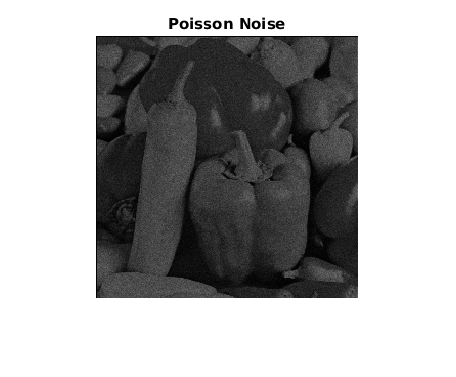
\includegraphics[scale=0.5]{images/peak100_noisy}
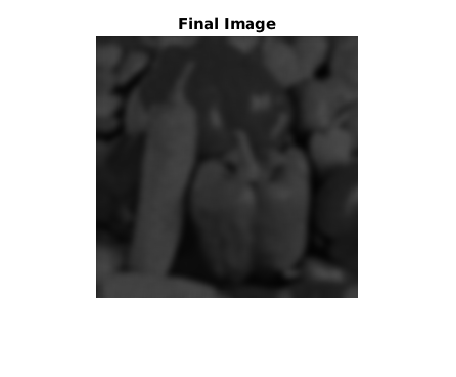
\includegraphics[scale=0.5]{images/peak100_denoised}
\\
PSNR\textsubscript{denoised} = 20.295 dB\\
\\
PSNR\textsubscript{noisy} = 19.093 dB
\end{document}
